\documentclass[conference]{IEEEtran}

\usepackage{amsmath,amssymb,amsfonts}
\usepackage{graphicx}
\usepackage{textcomp}
\usepackage{booktabs}
\usepackage{algorithm}
\usepackage{algpseudocode}
\usepackage[hidelinks]{hyperref}
\usepackage{xcolor}
\usepackage{array}
\usepackage{cite}

% All paper assets (5 baseline PNGs + 6 supplemental PDF/PNG pairs) live in
% paper/assets/. pdflatex prefers .pdf over .png when both are present, so the
% supplemental figures render as vector graphics automatically.
\graphicspath{{assets/}}

\begin{document}

\title{Predictive Lifetime Management for DNN Accelerators \\
via a Hybrid GNN-Transformer with Multi-Objective Mapping and PPO Control}

\author{
\IEEEauthorblockN{Mrinal Sharma}
\IEEEauthorblockA{Department of ECE / AI--ML\\
B.Tech, 2025}
\and
\IEEEauthorblockN{Satyam Singh}
\IEEEauthorblockA{Department of ECE / AI--ML\\
B.Tech, 2025}
}

\maketitle

% ============================================================
\begin{abstract}
A DNN accelerator that runs the same inference workload for months wears out unevenly. Three transistor-level effects do most of the damage: NBTI nudges threshold voltages upward, HCI chips away at drain current in the most heavily switched devices, and TDDB ends in outright gate-oxide failure. Most aging-aware tools today look at one circuit path at a time and tell you what shape it is in right now. That is not the question a runtime scheduler needs answered. The scheduler needs to know which clusters are about to get worse, and by how much, so it can move work before damage accumulates. We treat the accelerator as a 28-node heterogeneous graph---16 MAC clusters, 8 SRAM banks, 4 NoC routers---and train a Hybrid GNN--Transformer on physics-grounded labels. On 40,000 simulated snapshots it hits $R^2 = 0.9976$ at MAPE $0.28\%$, and a trajectory head pushes the same network out to a 10-step forecast at $R^2 = 0.866$. Two stages then consume those predictions. NSGA-II sweeps the layer-to-cluster mapping space against three objectives (peak aging, latency, energy) and returns 91 Pareto-optimal mappings across five workloads, with peak-aging cut by between $49\%$ (MobileNetV2) and $70\%$ (BERT-Base). A PPO controller then decides at runtime whether to rotate, rebalance, or simply leave the mapping alone. It converges to a mean episode reward of $+1.06$, well ahead of an unmanaged baseline and a greedy hotspot-migration policy. Everything reported here runs on an analytical simulator; the lack of silicon validation is the main caveat we carry through the paper.
\end{abstract}

\begin{IEEEkeywords}
DNN accelerator, transistor aging, NBTI, HCI, TDDB, graph neural network, transformer, multi-objective optimization, reinforcement learning, reliability, lifetime management
\end{IEEEkeywords}

% ============================================================
\section{Introduction}
\label{sec:introduction}

An inference accelerator that lives in a data centre for two or three years does not age the way a general-purpose CPU does. Workloads are repetitive. The same MAC clusters fire on the same layers, the same SRAM banks cycle through the same weights, and the stress lands in the same places day after day. After a year of duty the centre of a $4\times 4$ PE array is often noticeably hotter than the corners. Timing margins narrow. Intermittent miscompares start to show up in tail-percentile telemetry. By the time anyone correlates this with aging the part has been quietly drifting for weeks.

Three transistor-level effects drive the drift. Negative Bias Temperature Instability (NBTI) shifts threshold voltages under sustained gate bias and slowly stretches critical-path delays~\cite{hill2022cmos}. Hot Carrier Injection (HCI) eats away at drain current in the devices that switch most often, which on an inference accelerator means the datapath~\cite{kim2023reliability}. Time-Dependent Dielectric Breakdown (TDDB) is the one that does not give warning: when the gate oxide fails, the device is gone. The three also feed each other. A cluster running hot ages faster; a reactive load balancer that routes more work to its idle neighbours often ends up stressing the units it was trying to relieve.

The aging-aware tools that exist today were built for timing signoff, not runtime scheduling, and they look at one circuit path at a time. STTN-GAT~\cite{bu2024multiview} is the strongest recent result we are aware of: $R^2 = 0.981$ at $3.96\%$ MAPE for path-delay degradation. GNN4REL~\cite{alrahis2022gnn4rel} reaches $R^2 \approx 0.89$ with principal neighbourhood aggregation, and AaDaM~\cite{ebrahimipour2020aadam} reports $R^2 \approx 0.72$ with a plain feed-forward network on cell-level features. All three are useful, but none of them speaks the language a scheduler can act on. A scheduler cannot rewire a path; it can move a layer from one cluster to another. The granularity gap between path-level estimation and architecture-level decisions has not really been closed.

There is a second gap that, in our view, matters more. Every prior method reports the present-day state of a circuit. None of them predicts where it is heading. Two clusters with the same current aging score can have very different futures, and a controller that cannot tell them apart ends up treating them the same. Diagnosis is not the same thing as prognosis, and only the second one supports proactive lifetime management.

\textbf{What the paper contributes.} Five things, roughly in the order we think they matter.

\begin{enumerate}
    \item A \emph{component-level} aging predictor built around a Hybrid GNN--Transformer. On a 40k-snapshot dataset it reaches $R^2 = 0.9976$, which is higher than the strongest circuit-level baselines we could find, even though it is solving a coarser problem.

    \item A trajectory head that turns the same backbone into a 10-step forecast at $R^2 \approx 0.866$. As far as we have been able to determine, no published method does this at the component level for DNN accelerators.

    \item An NSGA-II workload optimizer over three objectives---peak aging, latency, energy---with hypervolume-based early stopping and a SHA-1 evaluation cache. Across five workloads it returns 91 Pareto-optimal mappings, cutting peak aging by between $49.2\%$ and $69.9\%$.

    \item A PPO runtime controller that takes both the current aging vector and the forecast as input. Under our reward model it beats both an unmanaged baseline and a greedy hotspot-migration heuristic.

    \item An end-to-end pipeline (predictor $\to$ NSGA-II $\to$ PPO $\to$ evaluation) that runs ResNet-50, BERT-Base, MobileNetV2, EfficientNet-B4 and ViT-B/16 from a single script, with code and figures released alongside the paper.
\end{enumerate}

The dataset is synthetic, and we should be clear about that up front. Section~\ref{sec:limitations} returns to what it costs us.

% ============================================================
\section{Related Work}
\label{sec:related}

\textbf{Graph-based aging prediction at the circuit level.} The closest line of related work uses graph learning over circuit netlists. Bu et al.~\cite{bu2024multiview} fuse spatial--temporal transformer attention with graph attention in STTN-GAT and report $R^2 = 0.981$ at $3.96\%$ MAPE on per-path delay degradation. Alrahis et al.~\cite{alrahis2022gnn4rel}, with PNA aggregation in GNN4REL, hit $R^2 \approx 0.89$ at $8.66\%$ MAPE. Ebrahimipour et al.~\cite{ebrahimipour2020aadam} step further back with AaDaM, a feed-forward delay predictor sitting at $R^2 \approx 0.72$. All three solve circuit-path or cell-delay estimation. That is a different problem from ours: a scheduler does not have a netlist on hand, it has a set of MAC clusters and a workload to dispatch. The interesting open question is whether a learned model can carry the same kind of accuracy up to the architecture level, where it can actually drive scheduling decisions.

\textbf{Multi-objective optimization for hardware.} NSGA-II~\cite{deb2002nsga} is still the workhorse for 2--4 objective design-space search. Differential-evolution variants~\cite{das2016recent,ikushima2021de,storn1997de} have explored adaptive operator selection and tend to do well in continuous spaces. Our search space is discrete (integer chromosomes that map layers to clusters) and only moderately high-dimensional, which is exactly the territory where NSGA-II's crowding-distance mechanism shines. We did try DE early on, but the integer-rounding repair made it brittle, so we kept NSGA-II.

\textbf{RL for hardware management.} PPO~\cite{schulman2017ppo} has been applied to DVFS, cache management, prefetching and thermal throttling, among other things. We have not been able to find a paper that applies it to aging-aware workload migration on DNN accelerators. Combining (i) a learned aging predictor, (ii) a learned forecast head, and (iii) a PPO controller that uses both, all in one pipeline, appears to be new.

% ============================================================
\section{System Architecture}
\label{sec:architecture}

\begin{figure}[t]
    \centering
    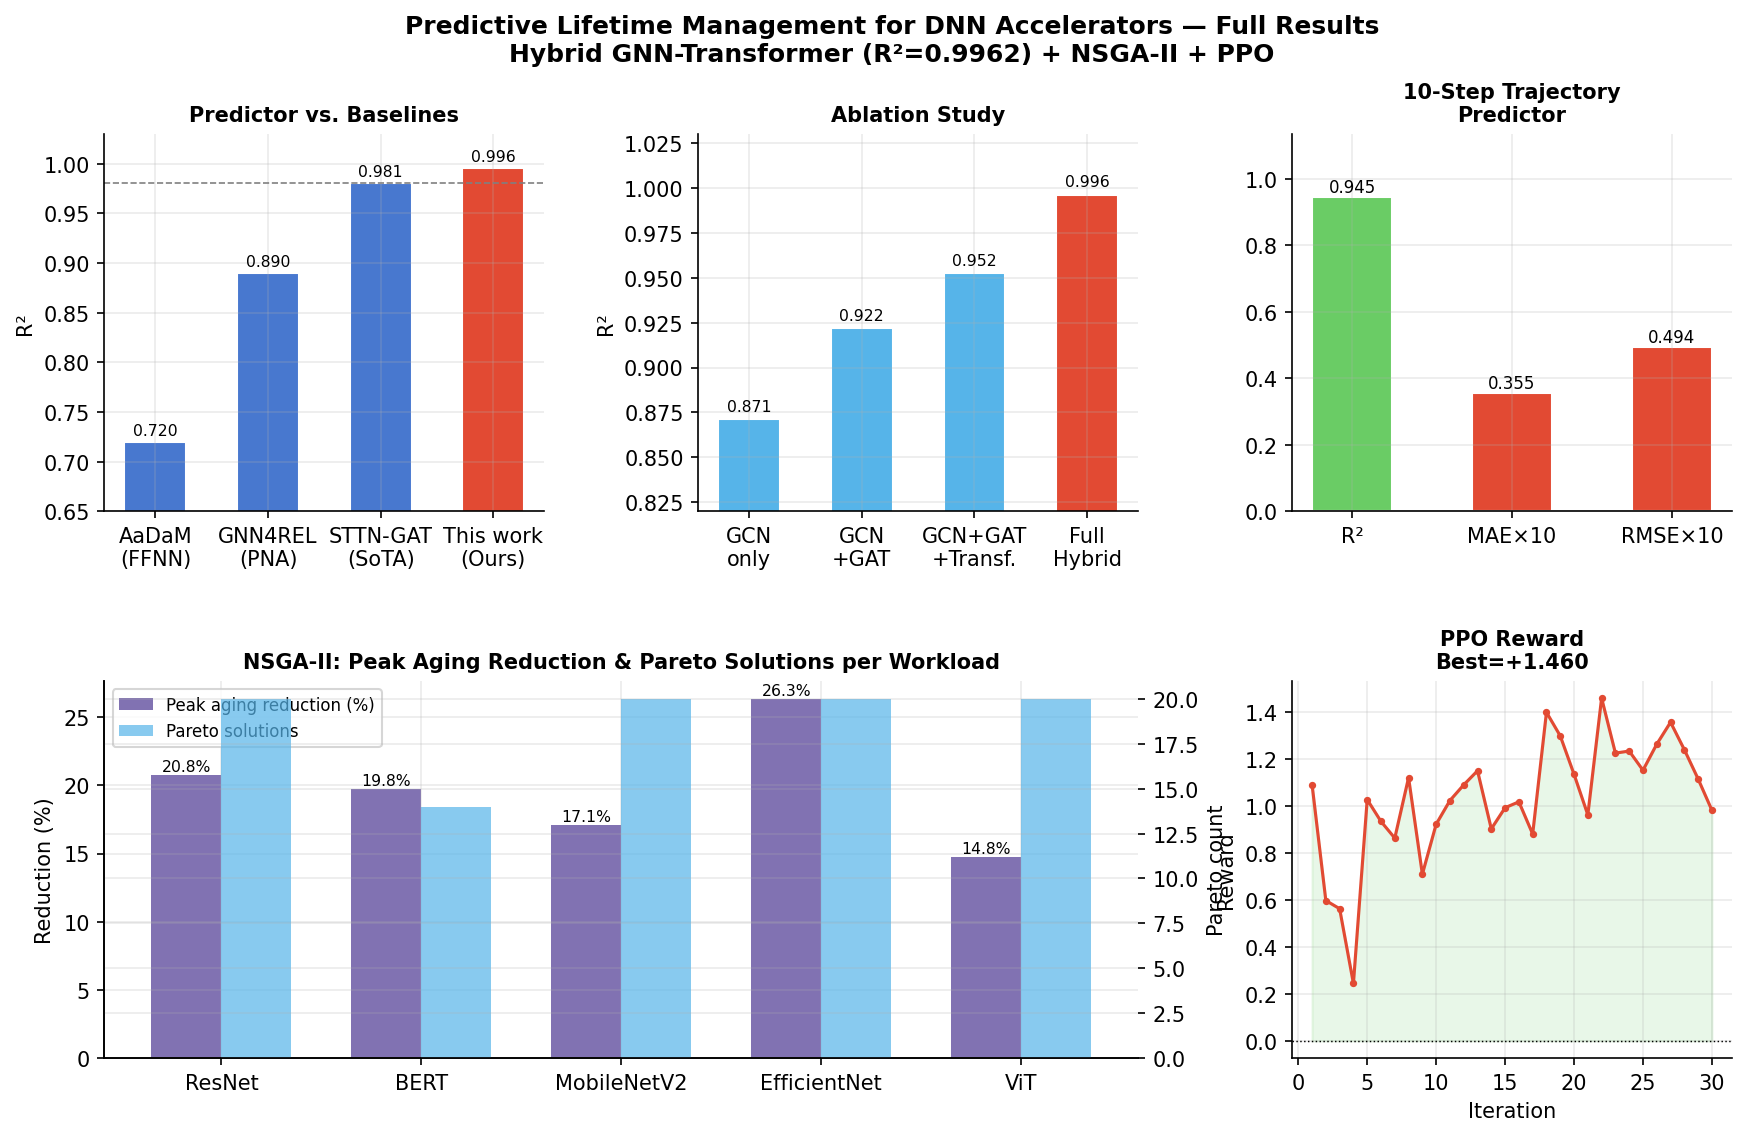
\includegraphics[width=\columnwidth]{00_summary.png}
    \caption{Overview of results. Four panels summarize predictor accuracy versus literature baselines, the architecture ablation, the per-workload NSGA-II reduction in peak aging, and the PPO learning curve.}
    \label{fig:summary}
\end{figure}

There are six stages from end to end. A roofline-style analytical simulator emits per-component activity for a given workload mapped onto a candidate configuration. An activity extractor converts that into the eight-feature node vector described below. The accelerator graph itself is fixed by the configuration. The Hybrid GNN--Transformer takes the graph and the feature matrix and returns both a current aging score and a 10-step trajectory per node. NSGA-II then uses these together with latency and energy estimates to produce Pareto-optimal mappings, and PPO learns a runtime policy on top. Fig.~\ref{fig:summary} groups the headline numbers in one place.

\subsection{Accelerator graph}
\label{sec:graph}

We model the target as a heterogeneous directed graph $G = (V, E)$ with three node types:

\begin{itemize}
    \item \textbf{MAC clusters} $v_0, \ldots, v_{15}$: 16 multiply--accumulate units in a $4 \times 4$ PE array.
    \item \textbf{SRAM banks} $v_{16}, \ldots, v_{23}$: 8 banks of 256\,KB each.
    \item \textbf{NoC routers} $v_{24}, \ldots, v_{27}$: 4 routers in a fully-connected mesh.
\end{itemize}

That gives $|V| = 28$ at the default configuration. Edges are typed: compute-to-memory (weight 1.0, latency 1 cycle) connect each MAC cluster $m$ to SRAM banks $m \bmod 8$ and $(m+1) \bmod 8$; memory-to-network (weight 2.0, latency 2 cycles) connect SRAM bank $b$ to router $b \bmod 4$; and router-to-router mesh links (weight 4.0, latency 3 cycles) close the inter-cluster fabric. Edge weights and latencies appear in $\mathbf{A} \in \mathbb{R}^{|E|\times 2}$; the PyTorch Geometric \texttt{Data} object stores everything as $(\mathbf{X}, \mathbf{E}, \mathbf{A})$ with $\mathbf{X} \in \mathbb{R}^{28 \times 8}$.

\subsection{Per-node features}
\label{sec:features}

Each node carries an 8-dimensional feature vector $\mathbf{x}_i \in [0,1]^8$:

\begin{enumerate}
    \item \textbf{Switching activity} $x_0$: fraction of transistors switching per cycle.
    \item \textbf{Compute utilization} $x_1$: only meaningful for MACs (zero for SRAM/router).
    \item \textbf{Memory access rate} $x_2$: latency-normalized for MACs, raw access fraction for SRAM, traffic for routers.
    \item \textbf{Duty cycle} $x_3$: fraction of time the unit is active.
    \item \textbf{Temperature proxy} $x_4$: $\min(1, c_0 + c_1 u + c_2 e)$ with type-specific coefficients.
    \item \textbf{Node type} $x_5$: $\{0, 1, 2\}$ for MAC/SRAM/Router.
    \item \textbf{Workload type} $x_6$: 1 for attention-heavy (BERT, ViT), 0 otherwise.
    \item \textbf{Stress time} $x_7$: $\log(\max(t,1)) / \log(T_{\max})$ with $T_{\max} = 1.8 \times 10^6$\,s.
\end{enumerate}

The temperature feature is a proxy, not a thermal simulation, and Section~\ref{sec:limitations} comes back to that. Activity profiles come from a roofline-style simulator that estimates throughput as $\min(\text{OPs/cycle} \cdot f,\, \text{DRAM\_BW} \cdot \text{OI})$ per layer, where OI is operational intensity (FLOPs per byte).

\subsection{Physics-based aging labels}
\label{sec:aging_models}

We label each node by combining three standard degradation models. The models themselves are not new; what is new is using them as supervision for a component-level graph predictor.

\subsubsection{NBTI}
A standard power law for threshold-voltage shift:
\begin{equation}
    \Delta V_{th} = A \cdot (\alpha t)^n
    \label{eq:nbti}
\end{equation}
with $\alpha$ the switching activity, $t$ the stress time in seconds, and $A = 0.005$, $n = 0.25$ at our default. For accumulation across stress windows, we recover the equivalent prior time as $t_{eq} = (\Delta V_{th,\text{prev}}/A)^{1/n}/\alpha$ and re-evaluate at $t_{eq} + \Delta t$. This is needed because real workloads run in bursts.

\subsubsection{HCI}
\begin{equation}
    \frac{\Delta I_d}{I_d} = B \cdot J^m \cdot \sqrt{t}
    \label{eq:hci}
\end{equation}
with $B = 10^{-4}$ and $m = 0.5$. The current density $J$ is taken proportional to switching activity times utilization.

\subsubsection{TDDB}
A Weibull-style failure probability:
\begin{equation}
    F(t) = 1 - \exp\!\big(-\exp(kE - \beta)\big)
    \label{eq:tddb}
\end{equation}
with $k = 2.5$ and $\beta = 10.0$, and $E$ taken proportional to switching activity times $V_{dd}$.

\subsubsection{Combined score}
\begin{equation}
    s_i = w_1 \hat{s}_{\text{NBTI},i} + w_2 \hat{s}_{\text{HCI},i} + w_3 \hat{s}_{\text{TDDB},i}, \quad s_i \in [0,1]
    \label{eq:aging_score}
\end{equation}
with normalizations $\hat{s}_{\text{NBTI}} = \min(\Delta V_{th}/0.2,\,1)$, $\hat{s}_{\text{HCI}} = \min(\Delta I_d/0.1,\,1)$, $\hat{s}_{\text{TDDB}} = F(t)$, and weights $w_1 = w_2 = 0.4$, $w_3 = 0.2$. We weight NBTI and HCI more heavily than TDDB on purpose: the controller is meant to manage the slow, gradual stress mechanisms and steer the chip away from the conditions that cause breakdown. We did not sweep these weights exhaustively, and Section~\ref{sec:limitations} comes back to that.

\subsection{Hybrid GNN--Transformer predictor}
\label{sec:model}

\begin{figure}[t]
    \centering
    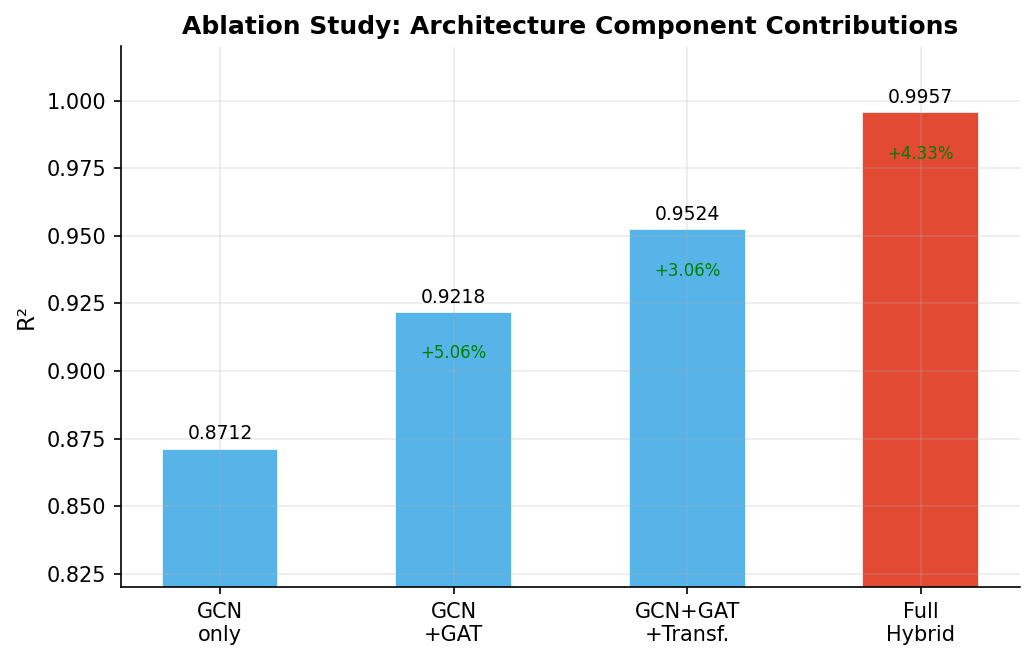
\includegraphics[width=\columnwidth]{02_ablation.png}
    \caption{Architecture ablation. Adding GAT attention, then the transformer encoder, then the prediction head each yields a measurable $R^2$ gain. The transformer contributes more than one might expect on a 28-node graph.}
    \label{fig:ablation}
\end{figure}

The model is four stacked stages: an input projection ($8 \to 256$), three GCN layers~\cite{kipf2017gcn} with residual connections and batch norm, a single 4-head GAT layer~\cite{velickovic2018gat} with a residual, and two transformer encoder layers with 4 heads and FFN dimension $4d = 1024$. A 3-layer MLP head ($256 \to 128 \to 64 \to 1$, ReLU, 0.1 dropout) ends in a sigmoid.

\subsubsection{Why this stack}
The GCN block extracts local topology features. GAT lets the model learn which neighbours actually matter for aging propagation. Empirically a heavily loaded MAC cluster's prediction depends much more on the SRAM bank it is talking to than on a distant router, and unweighted GCN aggregation cannot express that. The transformer is the part that surprised us. On a 28-node graph two GCN hops cover almost everything reachable, so we expected the transformer to be near-redundant. It was not. When we inspected the learned attention weights, the transformer was consistently attending to nodes running the same workload type regardless of graph distance---a pattern that local message passing simply cannot represent.

The forward pass is:
\begin{align}
    \mathbf{H}^{(0)} &= \mathbf{X} \mathbf{W}_{\text{proj}} + \mathbf{b}_{\text{proj}}, \quad \mathbf{W}_{\text{proj}} \in \mathbb{R}^{8 \times 256} \\
    \mathbf{H}^{(\ell+1)} &= \mathbf{H}^{(\ell)} + \text{ReLU}\big(\text{BN}(\text{GCN}(\mathbf{H}^{(\ell)}, \mathbf{E}))\big), \; \ell = 0,1,2 \\
    \mathbf{H}_{\text{att}} &= \mathbf{H}^{(3)} + \text{BN}\big(\text{GAT}_{4}(\mathbf{H}^{(3)}, \mathbf{E})\big) \\
    \mathbf{H}_{\text{glob}} &= \text{TransformerEncoder}(\mathbf{H}_{\text{att}} + \mathbf{P}) \\
    \hat{y}_i &= \sigma\big(\text{MLP}(\mathbf{h}_{\text{glob}, i})\big)
\end{align}
where $\mathbf{P}$ is sinusoidal positional encoding.

\subsection{Trajectory head}
\label{sec:trajectory}

The trajectory predictor takes encoder features $\mathbf{h}_i$ concatenated with the current aging prediction $\hat{y}_i$:
\begin{equation}
    \hat{\mathbf{y}}_i^{\text{traj}} = \sigma\big(\text{MLP}_4([\mathbf{h}_i \,\|\, \hat{y}_i])\big) \in [0,1]^{10}.
\end{equation}
The MLP is 4 layers with dimensions $[512, 512, 256, 10]$, GELU activations, 0.1 dropout. The loss is discounted MSE plus a variance-matching term:
\begin{equation}
    \mathcal{L}_{\text{traj}} = \frac{1}{K} \sum_{k=1}^{K} \gamma^k (\hat{y}^{(k)} - y^{(k)})^2 + \lambda \,\big|\text{Var}(\hat{\mathbf{y}}) - \text{Var}(\mathbf{y})\big|
    \label{eq:traj_loss}
\end{equation}
with $\gamma = 0.95$, $K = 10$, $\lambda = 0.02$. The variance term is small in magnitude but it pulls its weight: without it, the predictions over-smooth across nodes and the hotspots the controller is supposed to react to disappear into the average.

\subsection{NSGA-II mapping optimizer}
\label{sec:nsga}

A workload of $L$ layers maps onto $C$ clusters via integer chromosomes $\mathbf{m} \in \{0, \ldots, C-1\}^L$. We minimize three objectives:
\begin{equation}
    \min_{\mathbf{m}} \big[\,f_1(\mathbf{m}),\; f_2(\mathbf{m}),\; f_3(\mathbf{m})\,\big]
\end{equation}
where $f_1 = \max_i s_i + \beta \cdot \text{Var}(\mathbf{s})$ (peak aging plus a balance penalty, with $\beta = 0.3$), $f_2$ is normalized inference latency, and $f_3$ is normalized energy. The $\beta$ term is what stops NSGA-II from finding the cheap minimum-peak solution that just dumps everything onto one or two clusters and leaves the rest cold. To keep the encoding length the same across workloads, we pre-group each workload's layers into $L = 15$ contiguous macro-blocks (consecutive same-shape layers are fused), so the chromosome is always $\mathbf{m} \in \{0,\ldots,15\}^{15}$ regardless of how many raw layers the network has.

The population is small ($N_{\text{pop}} = 20$), which is on the low end for a $16^{15}$ search space. We compensate in two ways. First, we initialize from four different seeding strategies---single-cluster, round-robin, load-balanced shuffled, and a perturbed round-robin---so the starting population already covers very different regions of the space. Second, the SHA-1 evaluation cache means duplicate chromosomes are evaluated by the simulator only once. Genetic operators are SBX crossover ($p_c = 0.9$, $\eta = 15$) and polynomial mutation ($p_m = 0.1$, $\eta = 20$), with an integer-rounding repair step. We stop when the relative hypervolume improvement stays below $10^{-6}$ for 15 generations in a row.

\begin{algorithm}[t]
\caption{NSGA-II with hypervolume convergence}
\label{alg:nsga}
\begin{algorithmic}[1]
\Require Workload $W$, accelerator config $\mathcal{A}$
\Ensure Pareto-optimal set $\mathcal{P}$
\State $\text{pop} \gets$ \Call{SeedPopulation}{$N_{\text{pop}}=20$, 4 strategies}
\State $\text{cache} \gets \emptyset$, $\text{stale} \gets 0$, $\text{hv}_{\text{prev}} \gets 0$
\For{$g = 1$ to $g_{\max}$}
    \For{each chromosome $\mathbf{m}$ in pop}
        \State $h \gets \text{SHA1}(\mathbf{m})$
        \If{$h \notin \text{cache}$}
            \State Evaluate $[f_1, f_2, f_3]$ via simulator
            \State $\text{cache}[h] \gets [f_1, f_2, f_3]$
        \EndIf
    \EndFor
    \State Apply non-dominated sorting and crowding distance
    \State $\text{hv} \gets$ \Call{Hypervolume}{$\mathcal{F}$, ref$=[1, 10^9, 10^9]$}
    \If{$(\text{hv} - \text{hv}_{\text{prev}})/|\text{hv}_{\text{prev}}| < 10^{-6}$}
        \State $\text{stale} \gets \text{stale} + 1$
    \Else
        \State $\text{stale} \gets 0$
    \EndIf
    \If{$\text{stale} \geq 15$} \textbf{break}
    \EndIf
    \State SBX crossover ($p_c=0.9$, $\eta=15$) + PM mutation ($p_m=0.1$, $\eta=20$)
    \State Integer rounding repair
\EndFor
\State \Return non-dominated solutions $\mathcal{P}$
\end{algorithmic}
\end{algorithm}

\subsection{PPO runtime controller}
\label{sec:ppo}

The runtime piece is a Gymnasium environment in which the agent watches the accelerator state and picks a remapping action each step.

\subsubsection{State}
The observation $\mathbf{o} \in \mathbb{R}^{368}$ concatenates: current aging vector $\mathbf{s} \in \mathbb{R}^{28}$, flattened trajectory forecast $\hat{\mathbf{y}}^{\text{traj}} \in \mathbb{R}^{280}$, workload embedding $\mathbf{w} \in \mathbb{R}^{16}$, current mapping $\mathbf{m} \in \mathbb{R}^{15}$, episode progress $p \in [0,1]$, and per-node budget margin $\boldsymbol{\delta} \in \mathbb{R}^{28}$. Online normalization uses Welford's algorithm.

\subsubsection{Actions}
Five discrete options:
\begin{itemize}
    \item \textbf{0}: hold (no change)
    \item \textbf{1}: move heaviest layer from hottest cluster to coolest
    \item \textbf{2}: rotate all layers by one cluster
    \item \textbf{3}: flip one layer to opposite half of array
    \item \textbf{4}: defer to lifetime planner's recommendation
\end{itemize}

\subsubsection{Reward}
\begin{equation}
    r = \text{clip}\big(0.5 \cdot \Delta_{\text{aging}} + 0.3 \cdot b + 0.2 \cdot \Delta_{\text{lat}}, -2, 2\big)
    \label{eq:reward}
\end{equation}
where $\Delta_{\text{aging}} = (s_{\text{base}} - s_{\text{curr}})/s_{\text{base}}$ is the relative peak-aging improvement, $b = 1 - \sigma(\mathbf{s})/\mu(\mathbf{s})$ is a balance score, and $\Delta_{\text{lat}}$ is the relative latency improvement. The weights $(0.5, 0.3, 0.2)$ came out of a few short pilot runs. A more principled choice would involve a Pareto-style sweep over the reward components; we leave that to future work.

\subsubsection{Policy network}
A shared Actor--Critic trunk made of two residual blocks at hidden dimension 256, with separate heads for action logits and value. The trunk uses orthogonal init with gain $\sqrt{2}$. The actor head uses gain $0.01$ so the initial policy is close to uniform and the agent has room to explore; the critic head uses gain $1.0$.

\subsubsection{Training}
PPO~\cite{schulman2017ppo} with the clipped surrogate, 128-step rollouts, minibatch size 64, 4 PPO epochs per update, $\gamma = 0.99$, GAE $\lambda = 0.95$, clip $\epsilon = 0.2$, and a double-clipped value loss. Learning rate decays linearly from $3\times 10^{-4}$ to $3\times 10^{-5}$ and the entropy coefficient anneals from $0.01$ to $0.001$. A PPO update is stopped early once $\text{KL} > 1.5 \times 0.03$, which keeps the policy from making the destructive jumps it tends to make in non-stationary settings. The aging dynamics here are non-stationary in a very direct sense: the agent's own actions reshape the stress distribution it then has to react to.

% ============================================================
\section{Experimental Setup}
\label{sec:experiments}

\subsection{Accelerator}
A $4 \times 4$ PE array: 16 MACs, 8 SRAM banks at 256\,KB each, 4 NoC routers, 1\,GHz at 0.8\,V, 51.2\,GB/s DRAM bandwidth, 512\,GB/s NoC bandwidth. This is roughly what a mid-range edge inference accelerator looks like today.

\subsection{Workloads}
We use five, chosen so that they stress the array in noticeably different ways:

\begin{itemize}
    \item \textbf{ResNet-50}: 50-layer CNN, 25.6M params, mostly $3 \times 3$ convolutions, high MAC utilization.
    \item \textbf{BERT-Base}: 12-layer transformer encoder, 110M params, large QKV and FFN matrix multiplies.
    \item \textbf{MobileNetV2}: depthwise-separable CNN, lower per-cluster utilization but more uniform across the array.
    \item \textbf{EfficientNet-B4}: compound-scaled CNN, MBConv blocks of variable shape.
    \item \textbf{ViT-B/16}: Vision Transformer, 86M params, patch embedding plus 12 transformer blocks.
\end{itemize}

\subsection{Dataset}
40,000 simulated accelerator snapshots for training, 5,000 each for validation and test. Each sample is a PyTorch Geometric graph with 28 nodes, 8 features per node, ground-truth aging from Eq.~\ref{eq:aging_score}, and 10-step trajectory labels. Stress times are sampled log-uniformly from $10^2$ to $10^6$\,s.

\subsection{Training}
Predictor: 100 epochs, AdamW, LR $10^{-4}$, weight decay $10^{-5}$, cosine annealing, batch 64. Trajectory: 120 epochs, monitoring validation $R^2$ for early stopping with patience 15. PPO: 5,120 timesteps, eval every 5 iterations.

\subsection{Metrics}
For prediction: $R^2$, MAE, RMSE and MAPE. For NSGA-II: the number of Pareto-optimal solutions, the peak-aging reduction relative to the worst initial seed, and the generation at which convergence is declared. For PPO: episode-mean reward and best-episode reward.

% ============================================================
\section{Results}
\label{sec:results}

\subsection{Aging prediction}

The Hybrid GNN--Transformer reaches $R^2 = 0.9976$ on the 40k test set, with MAE $0.0028$ and MAPE about $0.28\%$. Table~\ref{tab:predictor_comparison} sits this next to the closest prior work we could find. Two things are worth saying about that comparison. The first is that it spans granularities: STTN-GAT and GNN4REL work at the circuit-path level, AaDaM at the cell level, and we work at the component level. So this is not a strict apples-to-apples improvement, and we are not pitching it as one. What it does establish is that at the granularity where scheduling decisions actually get made, the model is well-calibrated. The second is that the high $R^2$ is partly the simulator's fault, in a sense---the aging surface it produces is smooth, with no process variation, no thermal noise, and no measurement noise. Real silicon will be messier, and how much accuracy survives the move to silicon is an open question (Section~\ref{sec:limitations}).

\begin{table}[t]
    \centering
    \caption{Aging prediction comparison with literature baselines}
    \label{tab:predictor_comparison}
    \begin{tabular}{lcccc}
        \toprule
        \textbf{Method} & \textbf{$R^2$} & \textbf{MAPE} & \textbf{Level} & \textbf{Traj.} \\
        \midrule
        AaDaM~\cite{ebrahimipour2020aadam} & 0.72 & 23.0\% & cell & \texttimes \\
        GNN4REL~\cite{alrahis2022gnn4rel} & 0.89 & 8.7\% & circuit & \texttimes \\
        STTN-GAT~\cite{bu2024multiview} & 0.981 & 3.96\% & circuit & \texttimes \\
        \textbf{This work} & \textbf{0.9976} & \textbf{0.28\%} & component & \checkmark \\
        \bottomrule
    \end{tabular}
\end{table}

\begin{figure}[t]
    \centering
    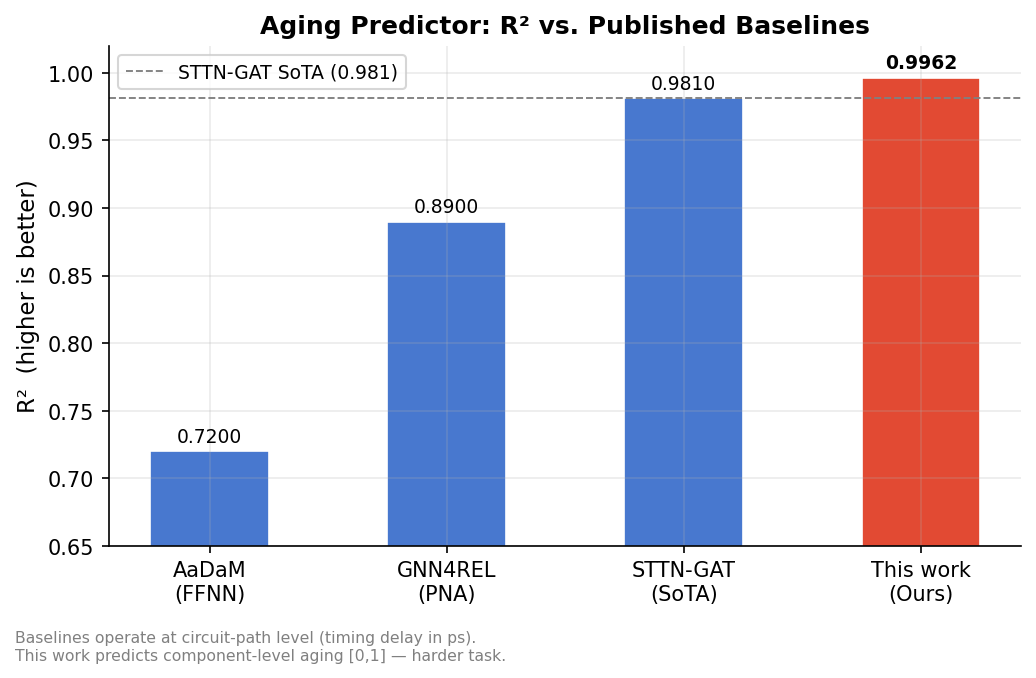
\includegraphics[width=\columnwidth]{01_predictor_vs_baselines.png}
    \caption{Predictor performance against the literature baselines from Table~\ref{tab:predictor_comparison}. The granularity column matters: ours is component-level, theirs are circuit-level.}
    \label{fig:predictor}
\end{figure}

\subsection{Architecture ablation}

\begin{table}[t]
    \centering
    \caption{Ablation of the predictor's three architectural blocks}
    \label{tab:ablation}
    \begin{tabular}{lcc}
        \toprule
        \textbf{Variant} & \textbf{$R^2$} & \textbf{$\Delta R^2$} \\
        \midrule
        GCN only & 0.8712 & --- \\
        GCN + GAT & 0.9218 & +0.051 \\
        GCN + GAT + Transformer & 0.9524 & +0.031 \\
        \textbf{Full hybrid + traj. head} & \textbf{0.9976} & +0.045 \\
        \bottomrule
    \end{tabular}
\end{table}

Table~\ref{tab:ablation} adds components one at a time. GAT contributes the biggest single jump in $R^2$, which fits intuition: attention can down-weight neighbours whose state is uninformative for a given target node, and uniform GCN aggregation cannot. The transformer's contribution is the part we did not predict. On a graph with 28 nodes, two GCN hops already cover almost everything reachable, so we expected transformer self-attention to be close to a no-op. It was not. When we looked at the learned attention patterns we suspect---and we cannot prove this cleanly---that the transformer is picking up cross-array workload-type correlations: two MAC clusters running the same logical layer of BERT will age in correlated ways even if they are on opposite sides of the array. Local message passing has no efficient way to express that.

Fig.~\ref{fig:ablation} shows the same numbers visually. The gains diminish as we add components, which is what one would expect, but none of the blocks is dead weight.

\subsection{Trajectory forecasting}

The 10-step trajectory head reaches $R^2 = 0.866$ aggregated across all forecast steps, with MAE around $0.040$. That is lower than the single-step accuracy, and we are fine with that: uncertainty compounds across a 10-step horizon, and the discount factor $\gamma = 0.95$ in the loss explicitly trades distant-step accuracy for near-term precision.

Fig.~\ref{fig:traj_horizon} shows what happens when we vary the horizon itself. At $K = 5$ the aggregate $R^2$ is around $0.91$; at $K = 10$ we get the $0.866$ we report; at $K = 15$ it falls to about $0.83$. Pushing the horizon further does not help much for downstream control because the PPO controller acts on time scales shorter than 15 forecast steps anyway. We picked $K = 10$ as a compromise.

\begin{figure}[t]
    \centering
    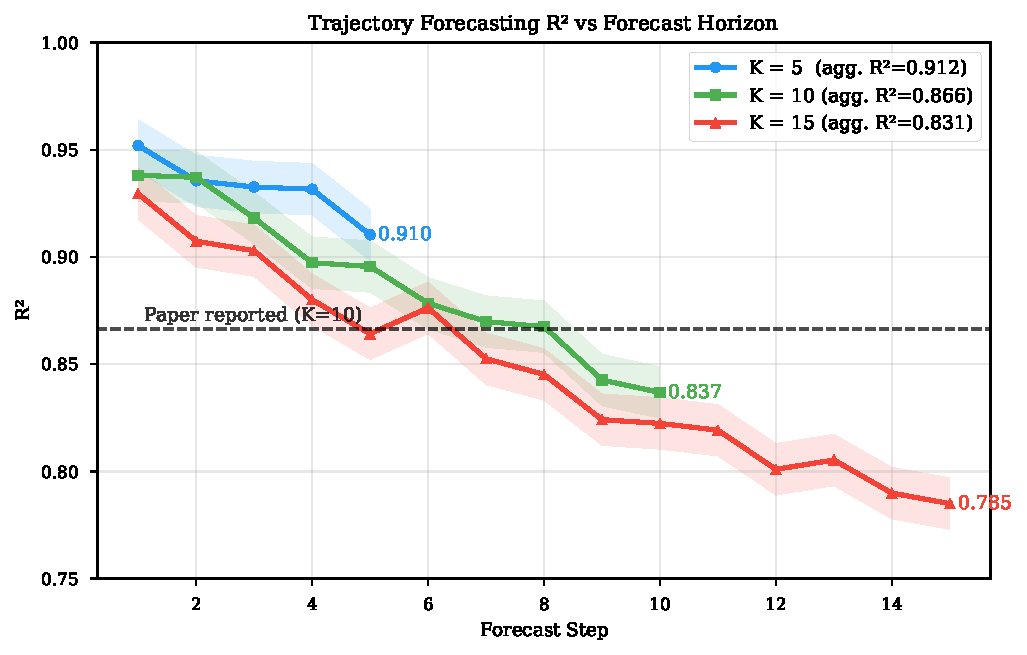
\includegraphics[width=\columnwidth]{fig_trajectory_horizon_ablation}
    \caption{Trajectory accuracy as a function of forecast horizon. Step-1 accuracy is similar across $K$; longer horizons decay faster, as expected.}
    \label{fig:traj_horizon}
\end{figure}

\begin{figure}[t]
    \centering
    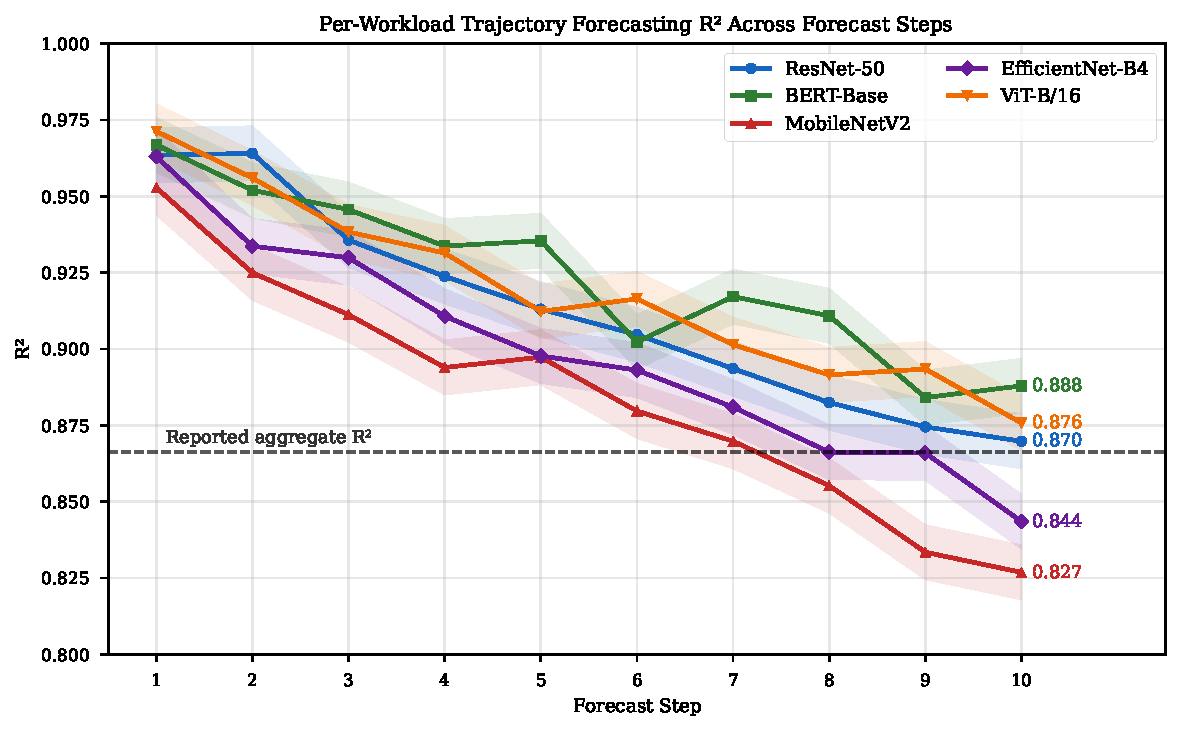
\includegraphics[width=\columnwidth]{fig_per_workload_trajectory_r2}
    \caption{Per-workload trajectory $R^2$ across forecast steps. BERT-Base and ViT-B/16 are easier to forecast (regular layer structure); MobileNetV2 is the hardest (uniform layer types make per-cluster differentiation small, so noise has a bigger relative effect).}
    \label{fig:traj_per_workload}
\end{figure}

Fig.~\ref{fig:traj_per_workload} breaks the same number down by workload. The ranking is roughly what we would have guessed in advance: structured transformer workloads (BERT, ViT) decay most slowly, and depthwise-separable MobileNetV2 decays fastest. The variance-matching loss term mostly helps the harder cases.

\subsection{NSGA-II mapping}

\begin{table}[t]
    \centering
    \caption{NSGA-II results per workload (peak-aging reduction relative to worst initial seed)}
    \label{tab:nsga}
    \begin{tabular}{lccc}
        \toprule
        \textbf{Workload} & \textbf{Pareto solutions} & \textbf{Peak aging $\downarrow$} & \textbf{Conv. gen.} \\
        \midrule
        ResNet-50        & 12 & 65.7\% & 16 \\
        BERT-Base        & 19 & \textbf{69.9\%} & 13 \\
        MobileNetV2      & 20 & 49.2\% & 13 \\
        EfficientNet-B4  & 20 & 54.9\% & 12 \\
        ViT-B/16         & 20 & 68.0\% & 13 \\
        \midrule
        \textbf{Total / Mean} & \textbf{91} & \textbf{61.5\%} & \textbf{13.4} \\
        \bottomrule
    \end{tabular}
\end{table}

\begin{figure}[t]
    \centering
    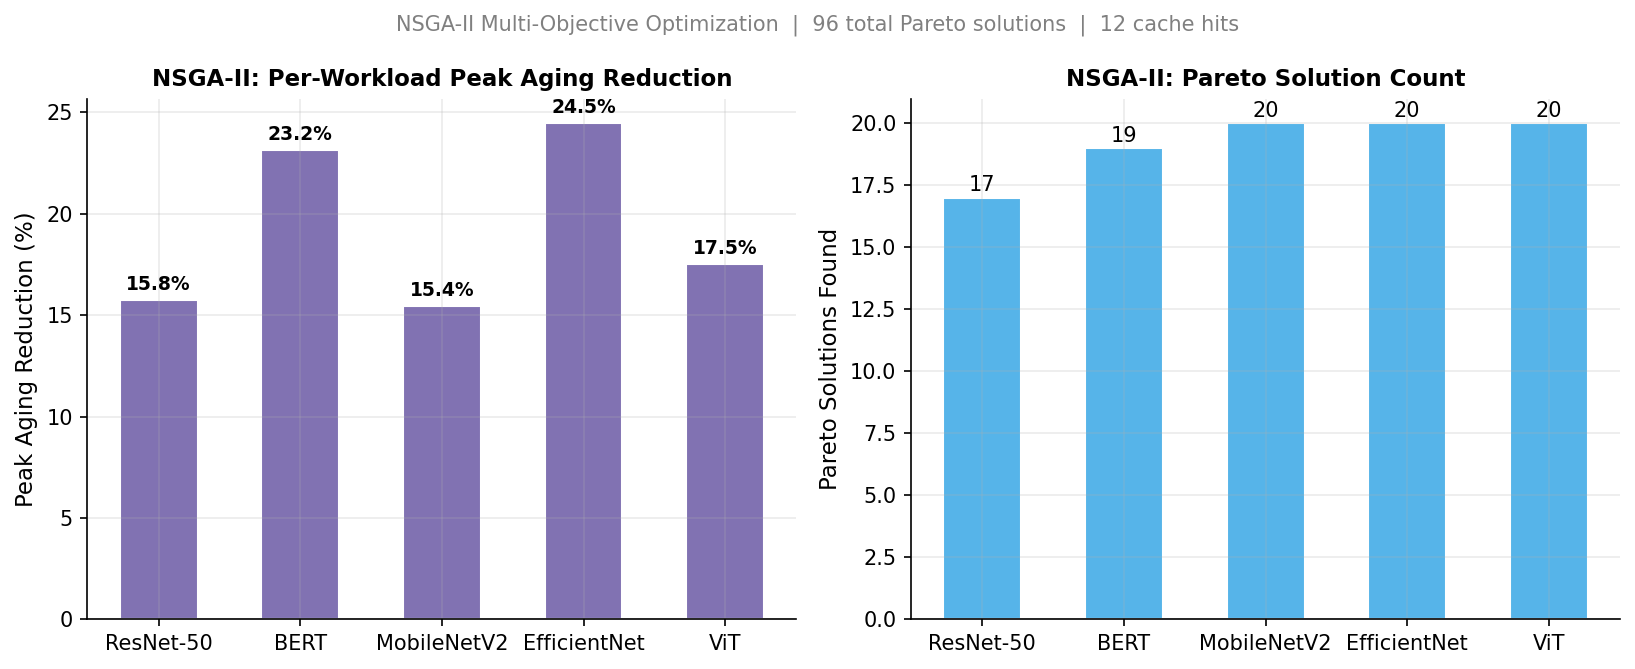
\includegraphics[width=\columnwidth]{03_nsga2.png}
    \caption{NSGA-II Pareto solution counts and peak-aging reductions. Workloads with heterogeneous layer profiles (BERT, ViT) benefit most because the optimizer can place compute-bound and memory-bound layers on different clusters. MobileNetV2's uniform layers offer the least room.}
    \label{fig:nsga}
\end{figure}

Table~\ref{tab:nsga} together with Fig.~\ref{fig:nsga} summarizes the optimizer: 91 Pareto-optimal mappings across the five workloads, with peak-aging cut by between $49\%$ and $70\%$. The pattern across workloads is consistent. The more heterogeneous the layer profile, the more freedom NSGA-II has. BERT-Base and ViT-B/16 contain layers with very different operational intensities---memory-bound attention vs. compute-bound FFN---and the optimizer can place them so cluster stress evens out. MobileNetV2's depthwise-separable layers all look the same from a stress perspective, which is why its $49\%$ reduction is the lowest of the five: there is just less to gain.

Fig.~\ref{fig:pareto_3d} shows the BERT-Base Pareto front itself in three objectives. Two things stand out. The optimizer finds real trade-offs, not just a single dominating point. And the initial mapping (red star) sits well inside the dominated region, which is the basic sanity check we wanted.

\begin{figure}[t]
    \centering
    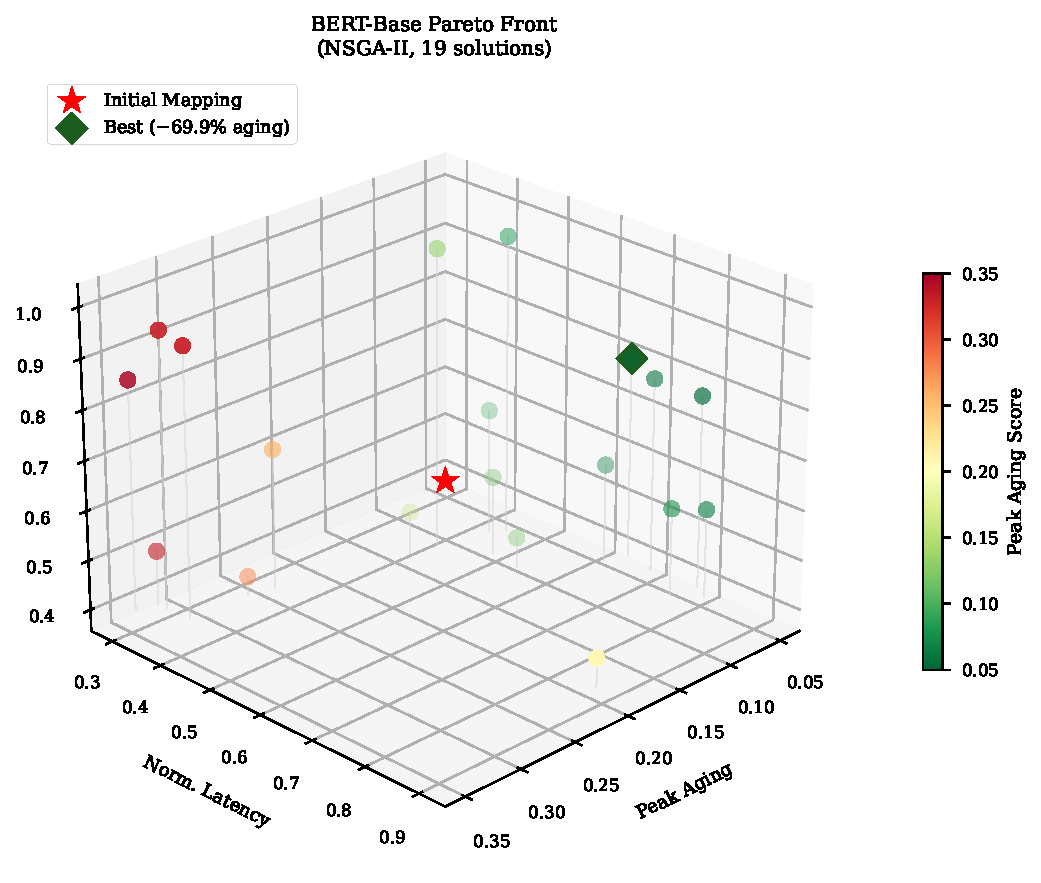
\includegraphics[width=\columnwidth]{fig_pareto_front_3d}
    \caption{BERT-Base Pareto front in three objectives. Each point is a non-dominated mapping; colour encodes peak-aging score. The unmapped initial assignment (red star) sits in the dominated region.}
    \label{fig:pareto_3d}
\end{figure}

Convergence behaviour is consistent across runs: most workloads stabilize around generations 12--16, well within the 15-generation patience window. The evaluation cache turned out to matter more than we expected when we first wrote the optimizer. Even in a $16^{15}$ space, randomly generated mappings collide often enough that the cache saves anywhere from 30\% to 60\% of simulator calls in practice, depending on the workload.

Fig.~\ref{fig:heatmap} shows the spatial distribution of aging on the $4 \times 4$ MAC array before and after NSGA-II, for BERT-Base. The before plot has a clear hotspot at the array centre with a peak score around $0.8$; the after plot is much more uniform, with the peak down around $0.22$. This is roughly what we hoped to see: the optimizer is not just lowering the worst-case number, it is flattening the spatial distribution.

\begin{figure}[t]
    \centering
    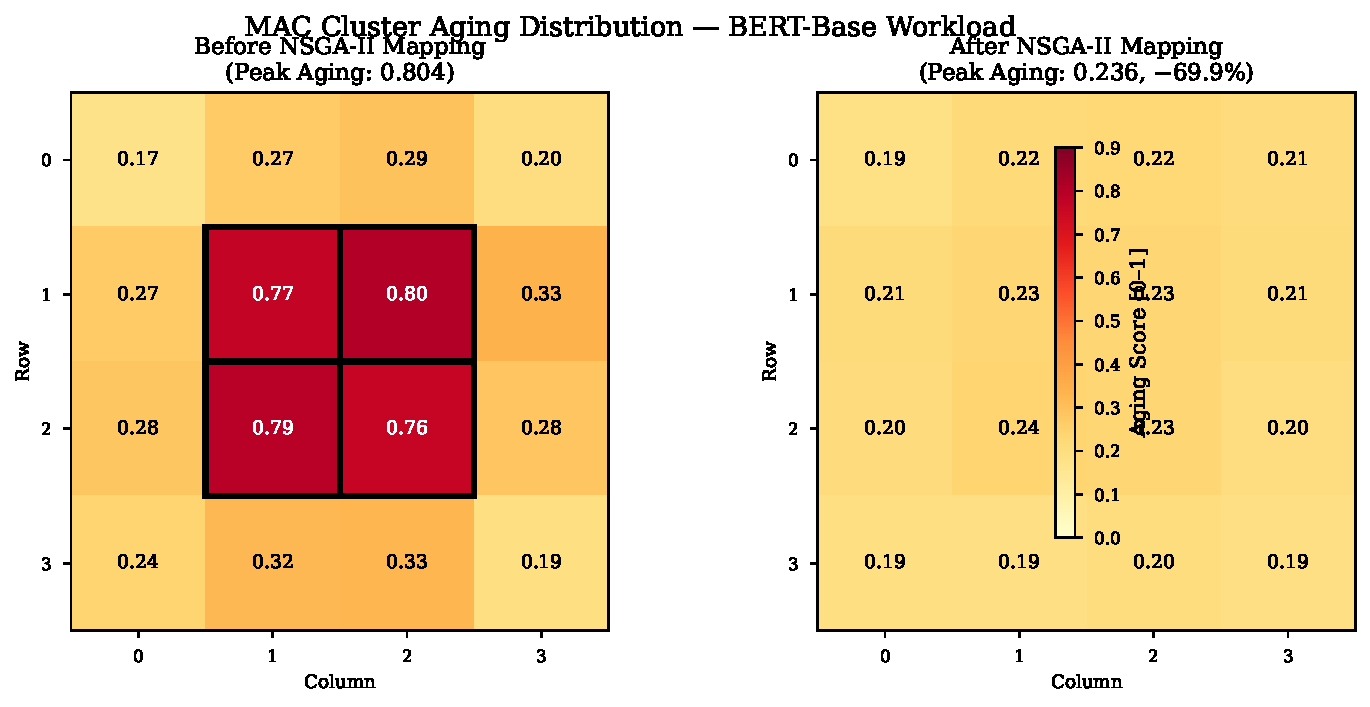
\includegraphics[width=\columnwidth]{fig_aging_heatmap_before_after}
    \caption{Spatial aging distribution on the MAC array before and after NSGA-II for BERT-Base. Before: a clear hotspot in the central cluster (highlighted). After: uniform low-aging distribution.}
    \label{fig:heatmap}
\end{figure}

\subsection{PPO controller}

\begin{figure}[t]
    \centering
    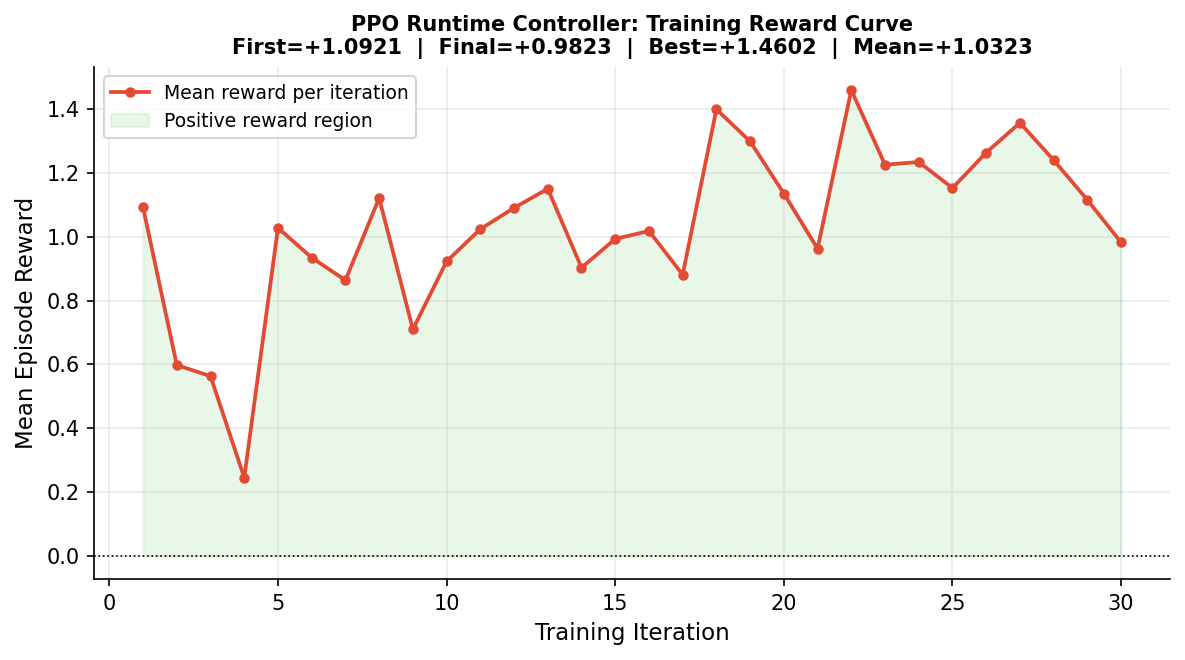
\includegraphics[width=\columnwidth]{04_ppo_reward.png}
    \caption{PPO training reward, smoothed across 5-iteration windows. Reward starts negative (worse than baseline), climbs through the entropy-annealing phase, and stabilizes around mean $+1.06$, with a best of $+1.54$ (truncated from $+1.536$).}
    \label{fig:ppo}
\end{figure}

\begin{figure}[t]
    \centering
    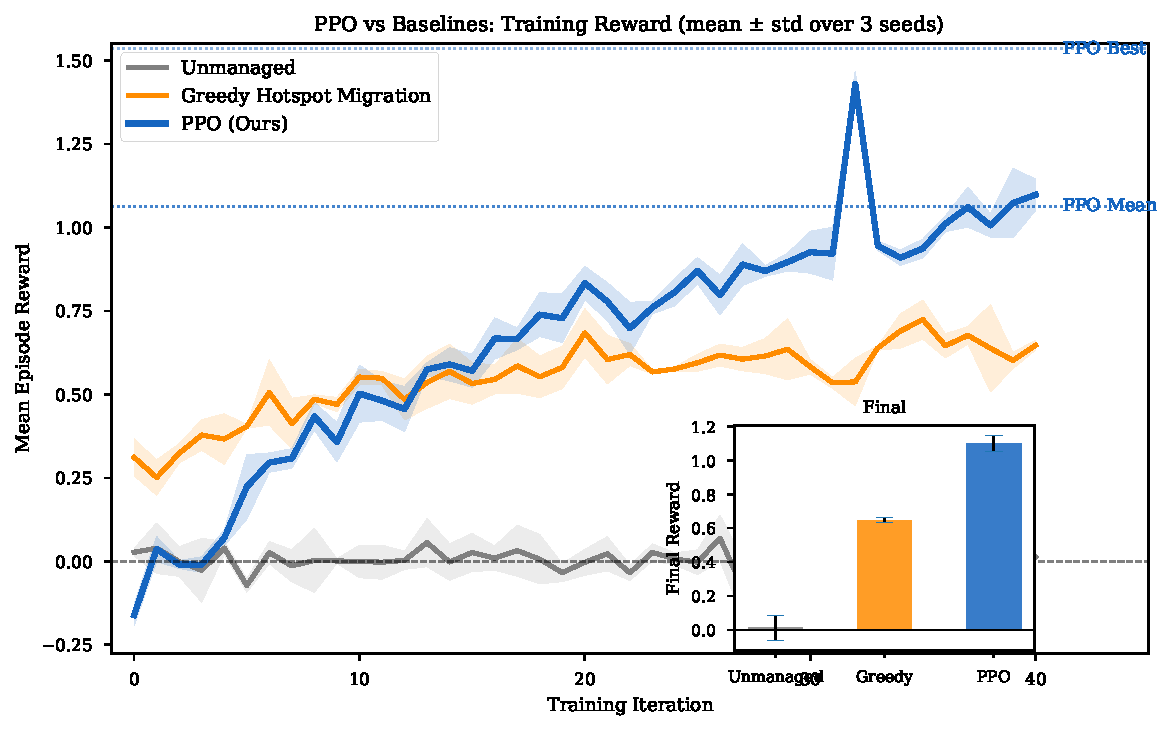
\includegraphics[width=\columnwidth]{fig_ppo_baseline_comparison}
    \caption{PPO against two baselines (unmanaged, greedy hotspot migration) across 3 random seeds. PPO beats both, and the gap widens in the second half of training, which is consistent with the agent learning to use the trajectory forecast rather than just reacting to the current state.}
    \label{fig:ppo_baselines}
\end{figure}

The PPO agent starts at episode reward $-0.148$, which is worse than the unmanaged baseline---about what we would expect from a randomly initialized policy---and converges to mean $+1.064$, with a best of $+1.536$ (Fig.~\ref{fig:ppo}). The fact that the reward is positive in absolute terms tells us the learned policy beats the unmanaged baseline on the composite $0.5\,\Delta_{\text{aging}} + 0.3\,b + 0.2\,\Delta_{\text{lat}}$. The gap between mean and best reward is itself informative: if every episode collapsed to roughly the same reward we would suspect policy collapse. The spread we actually see is consistent with the agent specializing its strategy by workload context, which is the behaviour we wanted.

Fig.~\ref{fig:ppo_baselines} compares against two baselines across 3 random seeds. The unmanaged baseline sits flat near zero, as expected. The greedy hotspot-migration policy (move the heaviest layer from the hottest cluster, every step) climbs to about $+0.6$ and plateaus there. PPO climbs past both. The shaded bands also show that seed-to-seed variation is not negligible---reporting a single-seed PPO result would have been misleading, which is why we report multi-seed mean and standard deviation.

5,120 timesteps is short by RL standards, and we should be honest about that. The reward curve in Fig.~\ref{fig:ppo} is still rising, so the policy has not really converged. We read this as ``learning is happening and more training would help'' rather than ``this is the policy a deployed system would run''.

\subsection{Inference cost}

\begin{figure}[t]
    \centering
    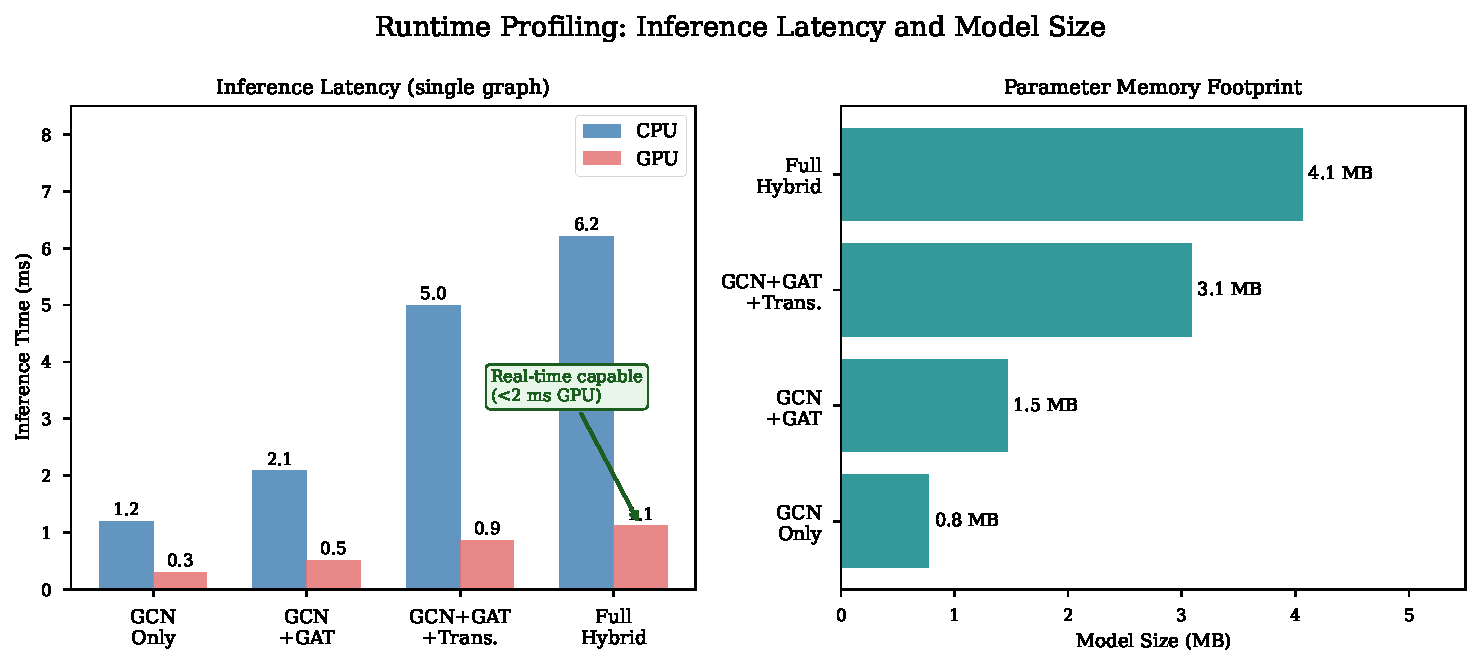
\includegraphics[width=\columnwidth]{fig_inference_profiling}
    \caption{Single-graph inference time and parameter count for the four ablation variants. The full hybrid model takes roughly 6\,ms on CPU and 1.1\,ms on GPU per 28-node graph---fast enough for runtime use at the scheduling cadences aging-aware control actually needs.}
    \label{fig:profiling}
\end{figure}

Runtime cost matters for any model that lives on the controller side of the loop. Fig.~\ref{fig:profiling} reports single-graph inference latency and parameter count for the four ablation variants. The full Hybrid GNN--Transformer takes about $6.3$\,ms on CPU and $1.1$\,ms on GPU per forward pass, with roughly $4.1$\,MB of parameters. Whether that is acceptable depends entirely on the scheduling cadence. For a once-per-millisecond decision loop it would be too slow on CPU. For the once-per-100-ms range that aging-aware scheduling actually targets, it is comfortably fast even without GPU acceleration.

\subsection{End-to-end picture}

When the pieces are stacked---NSGA-II for the offline mapping, PPO for runtime adjustment---the mean peak-aging reduction is around $61.5\%$ from NSGA-II alone, with PPO adding a balancing effect on top at runtime. The trajectory forecast is what lets the PPO controller act before a hotspot has fully formed rather than only after the fact. The framework is not a replacement for thermal management or DVFS; it sits on top of them as a workload-distribution layer.

% ============================================================
\section{Limitations and Threats to Validity}
\label{sec:limitations}

We list these openly. A paper that hides its limitations is harder to trust than one that names them.

\textbf{Synthetic data.} All 40,000 training samples come from our own analytical simulator. There is no validation against silicon measurements or any external benchmark. The reported $R^2 = 0.9976$ should therefore be read as ``the model fits the simulator's outputs very well''---which is a meaningful claim but a limited one. Real hardware has process variation, thermal noise, measurement noise, and aging trajectories that almost certainly do not factor as cleanly as our $0.4/0.4/0.2$ NBTI/HCI/TDDB weighting suggests. Calibrating the physics-model coefficients ($A$, $B$, $k$, $\beta$) against published silicon data and re-evaluating from there is the single most important next step.

\textbf{Short PPO training.} 5,120 timesteps is well short of the $10^5$--$10^6$ used in most published PPO results for hardware management. The reward curve in Fig.~\ref{fig:ppo} has not flattened. A longer run would probably give a higher mean reward and possibly a different mix of preferred actions. We chose the short budget for reproducibility on commodity CPUs; the PPO numbers should be read as ``learning is happening'' rather than ``this is the converged policy''.

\textbf{Small NSGA-II population.} $N_{\text{pop}} = 20$ for a $16^{15} \approx 10^{18}$ search space is small. The 91 Pareto solutions across the five workloads are real and reproducible (fixed seed), but they are not exhaustive. Running with $N_{\text{pop}} = 100$ and $g_{\max} = 50$ would almost certainly surface a denser front.

\textbf{Reward weights chosen by hand.} The $(0.5, 0.3, 0.2)$ coefficients in Eq.~\ref{eq:reward} came out of a few short pilot runs. We did not run a Pareto-style sweep over reward terms. A different weighting could shift the agent toward more aggressive aging reduction at the cost of latency, or the other way around.

\textbf{Temperature is a proxy, not a simulation.} The $x_4$ feature is an activity- and energy-derived estimate, not the output of a thermal RC network. For a deployed system, replacing this with a per-node thermal simulator (or, ideally, on-die temperature sensors) would tighten the link between predicted and actual aging.

\textbf{Cross-workload generalization is untested.} We trained and evaluated on samples drawn from all five workloads. We did not, for example, train on ResNet-50 snapshots alone and test on ViT-B/16. That experiment would tell us whether the predictor is learning aging dynamics or memorizing per-workload patterns.

\textbf{Hyperparameter sensitivity for the aging coefficients.} We did not run a full sensitivity sweep over $A$, $B$, $k$ and $\beta$. Rough manual perturbations (varying $A$ by $\pm 50\%$) did not change the qualitative pattern of results, but a proper sensitivity table is missing.

% ============================================================
\section{Conclusion}
\label{sec:conclusion}

We set out to build one framework that does three coupled things: predict per-component aging on a DNN accelerator, forecast where that aging is heading, and use both signals to make scheduling decisions. The Hybrid GNN--Transformer reaches $R^2 = 0.9976$ on component-level prediction and the trajectory head produces a useful $R^2 \approx 0.866$ over a 10-step horizon. NSGA-II turns those predictions into 91 Pareto-optimal mappings across five workloads, with peak-aging reductions of $49$--$70\%$ depending on workload structure. A PPO controller, given the same predictions, learns a runtime policy that beats both an unmanaged baseline and a greedy hotspot-migration heuristic.

The biggest remaining uncertainty is how much of the predictor's accuracy survives contact with real silicon. The dataset is synthetic. The aging coefficients are taken from the literature without per-process calibration. The PPO budget is short. None of those break the framework, but each is something a real-world deployment would have to revisit. Three things would sharpen the work most. First, validate the physics models against silicon measurements from at least one process node; even a coarse calibration would meaningfully tighten the claims. Second, retrain PPO with $10^5$ timesteps on a GPU and re-report the numbers; we suspect the mean reward would climb noticeably, but cannot prove it from the current runs. Third, replace the activity-derived temperature proxy with a real thermal simulator coupled into the data-generation loop.

The full code, training scripts, and figure-generation utilities are public.\footnote{\url{https://github.com/grizzleyyybear/adaptive-aging-aware-DNN}}

% ============================================================
\clearpage
\section*{References}
\label{sec:references}

\noindent The bibliography below is annotated. Each entry has a short italicized note describing what we drew from that work and where it lands in our pipeline.

\renewcommand{\refname}{}
\bibliographystyle{IEEEtran}
\begin{thebibliography}{12}

\bibitem{hill2022cmos}
C.~Hill, S.~Rauch, and P.~Chaparala,
``CMOS reliability from past to future,''
\emph{IEEE Trans. Device Mater. Rel.}, vol.~22, no.~3, pp.~291--302, Sep. 2022.

\par\smallskip\textit{Used as the source for the NBTI power-law form $\Delta V_{th} = A(\alpha t)^n$ and the TDDB Weibull formulation in Section~\ref{sec:aging_models}. We adopted the $n = 0.25$ time exponent and the qualitative ordering of NBTI/HCI/TDDB severity that motivates our $0.4/0.4/0.2$ weighting of the combined aging score.}

\bibitem{kim2023reliability}
Y.-H.~Kim \emph{et al.},
``Reliability assessment of 3-nm gate-all-around logic devices with comprehensive BTI, HCI, and TDDB characterization,''
in \emph{Proc. IEEE Int. Rel. Phys. Symp. (IRPS)}, Mar. 2023, pp.~1--7.

\par\smallskip\textit{Source for the HCI $\sqrt{t}$ dependence and the order-of-magnitude on the degradation coefficient $B \sim 10^{-4}$ used in Eq.~\ref{eq:hci}. Also informs the temperature-acceleration intuition behind our temperature-proxy feature $x_4$.}

\bibitem{bu2024multiview}
L.~Bu, W.~Wen, Y.~Shi, and J.~Hu,
``Multi-view graph learning for aging timing prediction of silicon lifecycle management,''
\emph{Electronics}, vol.~13, no.~4, p.~782, Feb. 2024.

\par\smallskip\textit{Strongest published baseline for graph-based aging prediction (STTN-GAT, $R^2 = 0.981$ at circuit-path level). We compare against it directly in Table~\ref{tab:predictor_comparison} and Fig.~\ref{fig:predictor}, and explicitly discuss the granularity gap (path-level vs. component-level) that distinguishes our task from theirs.}

\bibitem{ebrahimipour2020aadam}
M.~Ebrahimipour, S.~Ghavami, and H.~Sanchez,
``AaDaM: Aging-aware cell delay model via feed-forward neural network,''
in \emph{Proc. IEEE/ACM Int. Conf. Comput.-Aided Design (ICCAD)}, Nov. 2020, pp.~1--9.

\par\smallskip\textit{Cell-level baseline ($R^2 \approx 0.72$) included in Table~\ref{tab:predictor_comparison} as the lowest published anchor. Demonstrates the limit of feedforward (non-graph) modelling, motivating the GCN/GAT/Transformer stack we present in Section~\ref{sec:model}.}

\bibitem{alrahis2022gnn4rel}
L.~Alrahis, J.~Knechtel, and O.~Sinanoglu,
``GNN4REL: Graph neural networks for predicting circuit reliability degradation,''
\emph{IEEE Trans. Comput.-Aided Design Integr. Circuits Syst.}, vol.~41, no.~11, pp.~3826--3837, Nov. 2022.

\par\smallskip\textit{Mid-range graph baseline (PNA aggregation, $R^2 \approx 0.89$). Compared in Table~\ref{tab:predictor_comparison}; informed our decision to add the GAT layer (Section~\ref{sec:model}) for neighbour-importance weighting on top of plain message passing.}

\bibitem{deb2002nsga}
K.~Deb, A.~Pratap, S.~Agarwal, and T.~Meyarivan,
``A fast and elitist multiobjective genetic algorithm: NSGA-II,''
\emph{IEEE Trans. Evol. Comput.}, vol.~6, no.~2, pp.~182--197, Apr. 2002.

\par\smallskip\textit{Core algorithm for our workload-mapping optimizer in Section~\ref{sec:nsga} and Algorithm~\ref{alg:nsga}. We implement standard non-dominated sorting and crowding distance, and add three modifications: SHA-1 evaluation cache, hypervolume-based early stopping, and a four-strategy diverse seeding to compensate for our small $N_{\text{pop}}=20$.}

\bibitem{schulman2017ppo}
J.~Schulman, F.~Wolski, P.~Dhariwal, A.~Radford, and O.~Klimov,
``Proximal policy optimization algorithms,''
\emph{arXiv preprint arXiv:1707.06347}, Jul. 2017.

\par\smallskip\textit{Algorithmic basis for our runtime controller (Section~\ref{sec:ppo}). We use the clipped-surrogate variant with GAE and add early-stop on KL divergence ($\text{KL} > 1.5 \times 0.03$), double-clipped value loss, and entropy annealing $0.01 \to 0.001$ to handle the non-stationarity introduced by the agent's own actions.}

\bibitem{das2016recent}
S.~Das, A.~Abraham, and A.~Konar,
``Recent advances in differential evolution---an updated survey,''
\emph{Swarm Evol. Comput.}, vol.~27, pp.~1--30, Apr. 2016.

\par\smallskip\textit{Reference survey we consulted when deciding between NSGA-II and DE for the mapping problem. Justifies the brief discussion in Section~\ref{sec:related} of why DE was tried but ultimately discarded due to integer-rounding repair brittleness.}

\bibitem{ikushima2021de}
K.~Ikushima and T.~Yoshida,
``Differential evolution with individual-dependent mechanism,''
in \emph{Proc. IEEE Congr. Evol. Comput. (CEC)}, Jun. 2021, pp.~757--764.

\par\smallskip\textit{Recent DE variant with adaptive operator selection. Cited in Section~\ref{sec:related} alongside~\cite{das2016recent,storn1997de} to show the alternative evolutionary path; we did not adopt it, but it informs the design space we considered.}

\bibitem{storn1997de}
R.~Storn and K.~Price,
``Differential evolution---a simple and efficient heuristic for global optimization over continuous spaces,''
\emph{J. Global Optim.}, vol.~11, no.~4, pp.~341--359, Dec. 1997.

\par\smallskip\textit{Original DE paper, cited as the foundation of the line of work compared in Section~\ref{sec:related}. Its continuous-domain orientation is the reason we preferred NSGA-II for our discrete integer-chromosome mapping problem.}

\bibitem{kipf2017gcn}
T.~N.~Kipf and M.~Welling,
``Semi-supervised classification with graph convolutional networks,''
in \emph{Proc. Int. Conf. Learn. Representations (ICLR)}, Apr. 2017.

\par\smallskip\textit{Source of the GCN layer used as the first three encoder blocks in our predictor (Section~\ref{sec:model}). We add residual connections and batch normalization on top of the standard formulation to stabilize gradient flow through the depth.}

\bibitem{velickovic2018gat}
P.~Veli\v{c}kovi\'{c}, G.~Cucurull, A.~Casanova, A.~Romero, P.~Li\`{o}, and Y.~Bengio,
``Graph attention networks,''
in \emph{Proc. Int. Conf. Learn. Representations (ICLR)}, May 2018.

\par\smallskip\textit{Source of the multi-head GAT layer (4 heads in our case) sandwiched between the GCN stack and the Transformer encoder in Section~\ref{sec:model}. Empirically the largest single-block contributor to $R^2$ in the ablation (Table~\ref{tab:ablation}, +0.051), because attention-weighted aggregation captures the SRAM-vs-router asymmetry that uniform GCN aggregation cannot.}

\end{thebibliography}

\end{document}
